\documentclass[tikz,border=2pt]{standalone}
\usepackage[T1]{fontenc}\usepackage{helvet}\usepackage{amsmath}
% shared TikZ styles for the three block diagrams (editable sources)
\usetikzlibrary{arrows.meta,positioning,fit,calc,backgrounds,shapes.geometric}
\definecolor{learn}{HTML}{6250D6}   % learned components
\definecolor{numer}{HTML}{2A78D6}   % numerical methods (Kalman lineage)
\definecolor{numerh}{HTML}{EB6834}  % numerical methods (Khalil lineage)
\definecolor{check}{HTML}{1D6B43}   % deterministic checks
\definecolor{ink}{HTML}{1B2430}
\definecolor{mut}{HTML}{5D6B7A}
\tikzset{
  every node/.style={font=\sffamily\scriptsize,text=ink,execute at begin node={\hyphenpenalty=10000 \exhyphenpenalty=10000 }},
  box/.style={draw=mut,rounded corners=1.5pt,line width=0.5pt,align=center,inner sep=3.5pt,fill=white,minimum height=6.5mm},
  learned/.style={box,draw=learn,dashed,line width=0.8pt,fill=learn!7},
  numeric/.style={box,draw=numer,line width=0.8pt,fill=numer!7},
  numerich/.style={box,draw=numerh,line width=0.8pt,fill=numerh!8},
  checkb/.style={box,draw=check,line width=0.8pt,double,double distance=0.6pt,fill=check!6},
  user/.style={box,fill=black!5},
  arr/.style={-{Stealth[length=4pt,width=3.4pt]},line width=0.5pt,draw=ink},
  darr/.style={arr,dashed},
  lab/.style={font=\sffamily\fontsize{6}{7}\selectfont,text=mut,align=center},
  onl/.style={lab,fill=white,inner sep=1.5pt},
  group/.style={draw=mut,dotted,line width=0.6pt,rounded corners=3pt,inner sep=5pt},
}

% What remains human, and what remains open (closing section).  Colors as in the framework and pipeline figures:
% coordinator and checks green, Kalman specialist blue, Khalil specialist orange, learned reader violet (dashed),
% people gray.
\tikzset{every node/.append style={font=\sffamily\footnotesize},
         lab/.style={font=\sffamily\fontsize{7}{8}\selectfont,text=mut,align=center},
         head/.style={font=\sffamily\bfseries\fontsize{8.5}{10}\selectfont,text=ink,anchor=south west,inner sep=0pt},
         card/.style={text width=#1,align=left,inner sep=3.5pt,font=\sffamily\fontsize{7}{8.4}\selectfont},
         chip/.style={box,fill=check!6,draw=check,line width=0.6pt,text width=2.55cm,align=center,inner sep=2.5pt,
                      font=\sffamily\fontsize{7}{8.5}\selectfont,minimum height=5.2mm},
         dot/.style={circle,fill=ink,inner sep=0pt,minimum size=1.7mm}}
\begin{document}
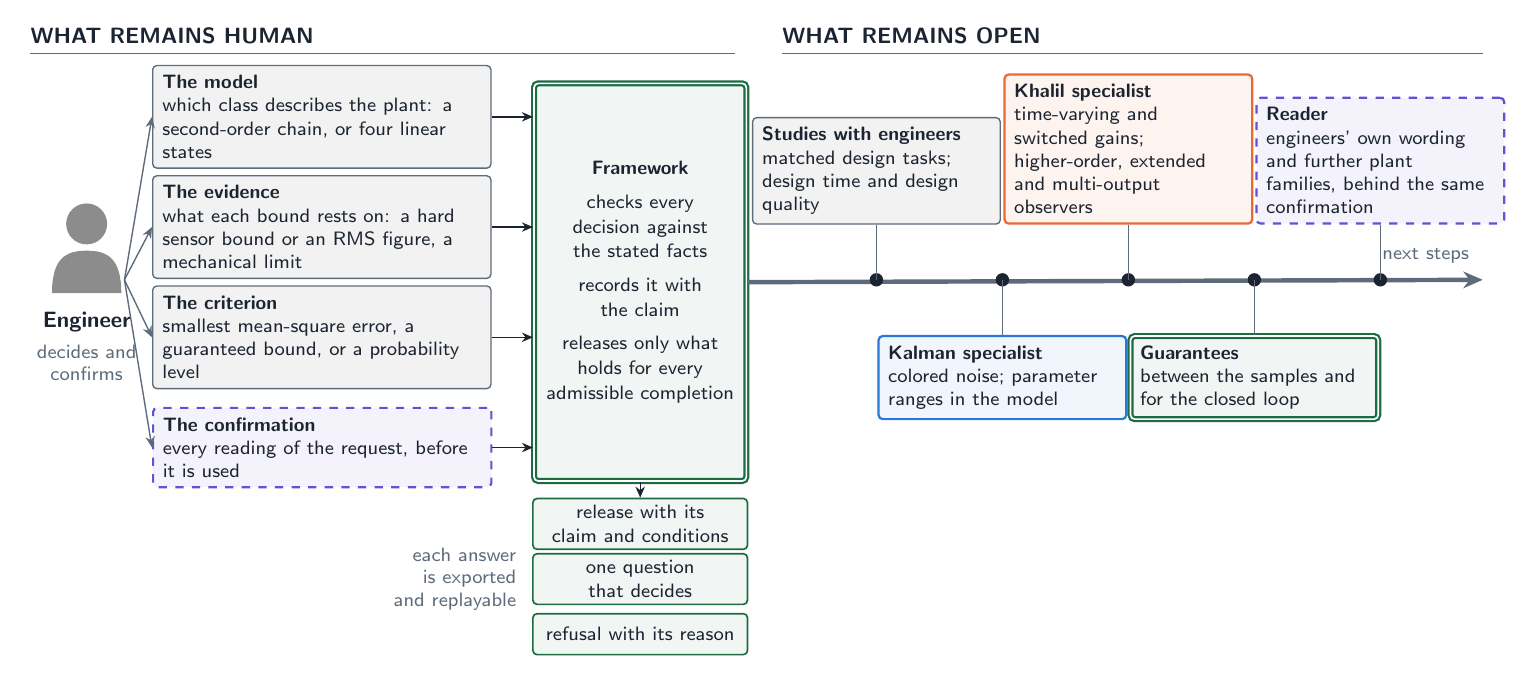
\begin{tikzpicture}[x=1cm,y=1cm]
% ===================== left: what remains human =====================
\node[head] at (0,6.55) {WHAT REMAINS HUMAN};
\draw[mut,line width=0.4pt] (0,6.42) -- (8.95,6.42);
% the engineer
\begin{scope}[shift={(0.72,3.7)}]
  \fill[black!45] (0,0.56) circle (0.26);
  \fill[black!45] (-0.44,-0.32) .. controls (-0.44,0.12) and (-0.27,0.22) .. (0,0.22)
                   .. controls (0.27,0.22) and (0.44,0.12) .. (0.44,-0.32) -- cycle;
\end{scope}
\node[font=\sffamily\bfseries\footnotesize,anchor=north,align=center] (eng) at (0.72,3.27) {Engineer};
\node[lab,anchor=north] at (0.72,2.85) {decides and\\ confirms};
% the four decisions
\node[user,card=4.05cm,anchor=west] (dm) at (1.55,5.62) {\textbf{The model}\\ which class describes the plant: a second-order chain, or four linear states};
\node[user,card=4.05cm,anchor=west] (de) at (1.55,4.22) {\textbf{The evidence}\\ what each bound rests on: a hard sensor bound or an RMS figure, a mechanical limit};
\node[user,card=4.05cm,anchor=west] (dc) at (1.55,2.82) {\textbf{The criterion}\\ smallest mean-square error, a guaranteed bound, or a probability level};
\node[learned,card=4.05cm,anchor=west] (dr) at (1.55,1.42) {\textbf{The confirmation}\\ every reading of the request, before it is used};
\foreach \d in {dm,de,dc,dr} \draw[arr,draw=mut] (1.2,3.55) -- (\d.west);
% the framework
\node[checkb,text width=2.45cm,align=center,minimum height=5.05cm,font=\sffamily\fontsize{7.5}{9}\selectfont] (fw) at (7.75,3.52) {\textbf{Framework}\\[3pt]
  checks every decision against the stated facts\\[3pt] records it with the claim\\[3pt]
  releases only what holds for every admissible completion};
\foreach \d in {dm,de,dc,dr} \draw[arr] (\d.east) -- (\d.east -| fw.west);
% what comes back
\node[chip] (o1) at (7.75,0.45) {release with its claim and conditions};
\node[chip] (o2) at (7.75,-0.25) {one question that decides};
\node[chip] (o3) at (7.75,-0.95) {refusal with its reason};
\draw[arr] (fw.south) -- (o1.north);
\node[lab,anchor=east,align=right] at (6.3,-0.25) {each answer\\ is exported\\ and replayable};
% ===================== right: what remains open =====================
\node[head] at (9.55,6.55) {WHAT REMAINS OPEN};
\draw[mut,line width=0.4pt] (9.55,6.42) -- (18.45,6.42);
\draw[-{Stealth[length=7pt,width=6pt]},line width=1.6pt,draw=mut] (fw.east |- 0,3.52) -- (18.45,3.55);
\node[lab,anchor=south east] at (18.4,3.63) {next steps};
\foreach \x in {10.75,12.35,13.95,15.55,17.15} \node[dot] at (\x,3.55) {};
% milestones, alternating above and below the arrow
\node[user,card=2.9cm,anchor=south] (s1) at (10.75,4.25) {\textbf{Studies with engineers}\\ matched design tasks; design time and design quality};
\node[numeric,card=2.9cm,anchor=north] (s2) at (12.35,2.85) {\textbf{Kalman specialist}\\ colored noise; parameter ranges in the model};
\node[numerich,card=2.9cm,anchor=south] (s3) at (13.95,4.25) {\textbf{Khalil specialist}\\ time-varying and switched gains; higher-order, extended and multi-output observers};
\node[checkb,card=2.9cm,anchor=north] (s4) at (15.55,2.85) {\textbf{Guarantees}\\ between the samples and for the closed loop};
\node[learned,card=2.9cm,anchor=south] (s5) at (17.15,4.25) {\textbf{Reader}\\ engineers' own wording and further plant families, behind the same confirmation};
\foreach \s/\x in {s1/10.75,s3/13.95,s5/17.15} \draw[mut,line width=0.6pt] (\x,3.55) -- (\s.south);
\foreach \s/\x in {s2/12.35,s4/15.55} \draw[mut,line width=0.6pt] (\x,3.55) -- (\s.north);
\end{tikzpicture}
\end{document}
